\chapter{Hopping Gait}
\label{chap:hopping_gait}

We plan to generate a stable hopping gait by utilizing the SLOM concept for the system designed in Chapter. 
\ref{chap:mech_design}. The strategy to do that would be to first derive the equations of the motion of the 
whole system and propagate them using correct constraints and event solvers. The initial part of this 
chapter addresses these issues. Once we can propagate these set of equations from any initial condition, we 
try to find a relation between the impact states of every hop. The variation of these impact states will 
enable us to find if the gait is stable or not. We will try to find out good sets of initial conditions 
such that the impact states do not change much i.e. impact states are the fixed point of the Poincare Map 
of the set of differential equations.\\

Next step in the analysis would be to devise a control strategy for attitude re--orientation. The spring 
extension controller is already devised while finding the impact states.

\section{Euler-Lagrange equations}
\begin{figure}[!htp]
\centering
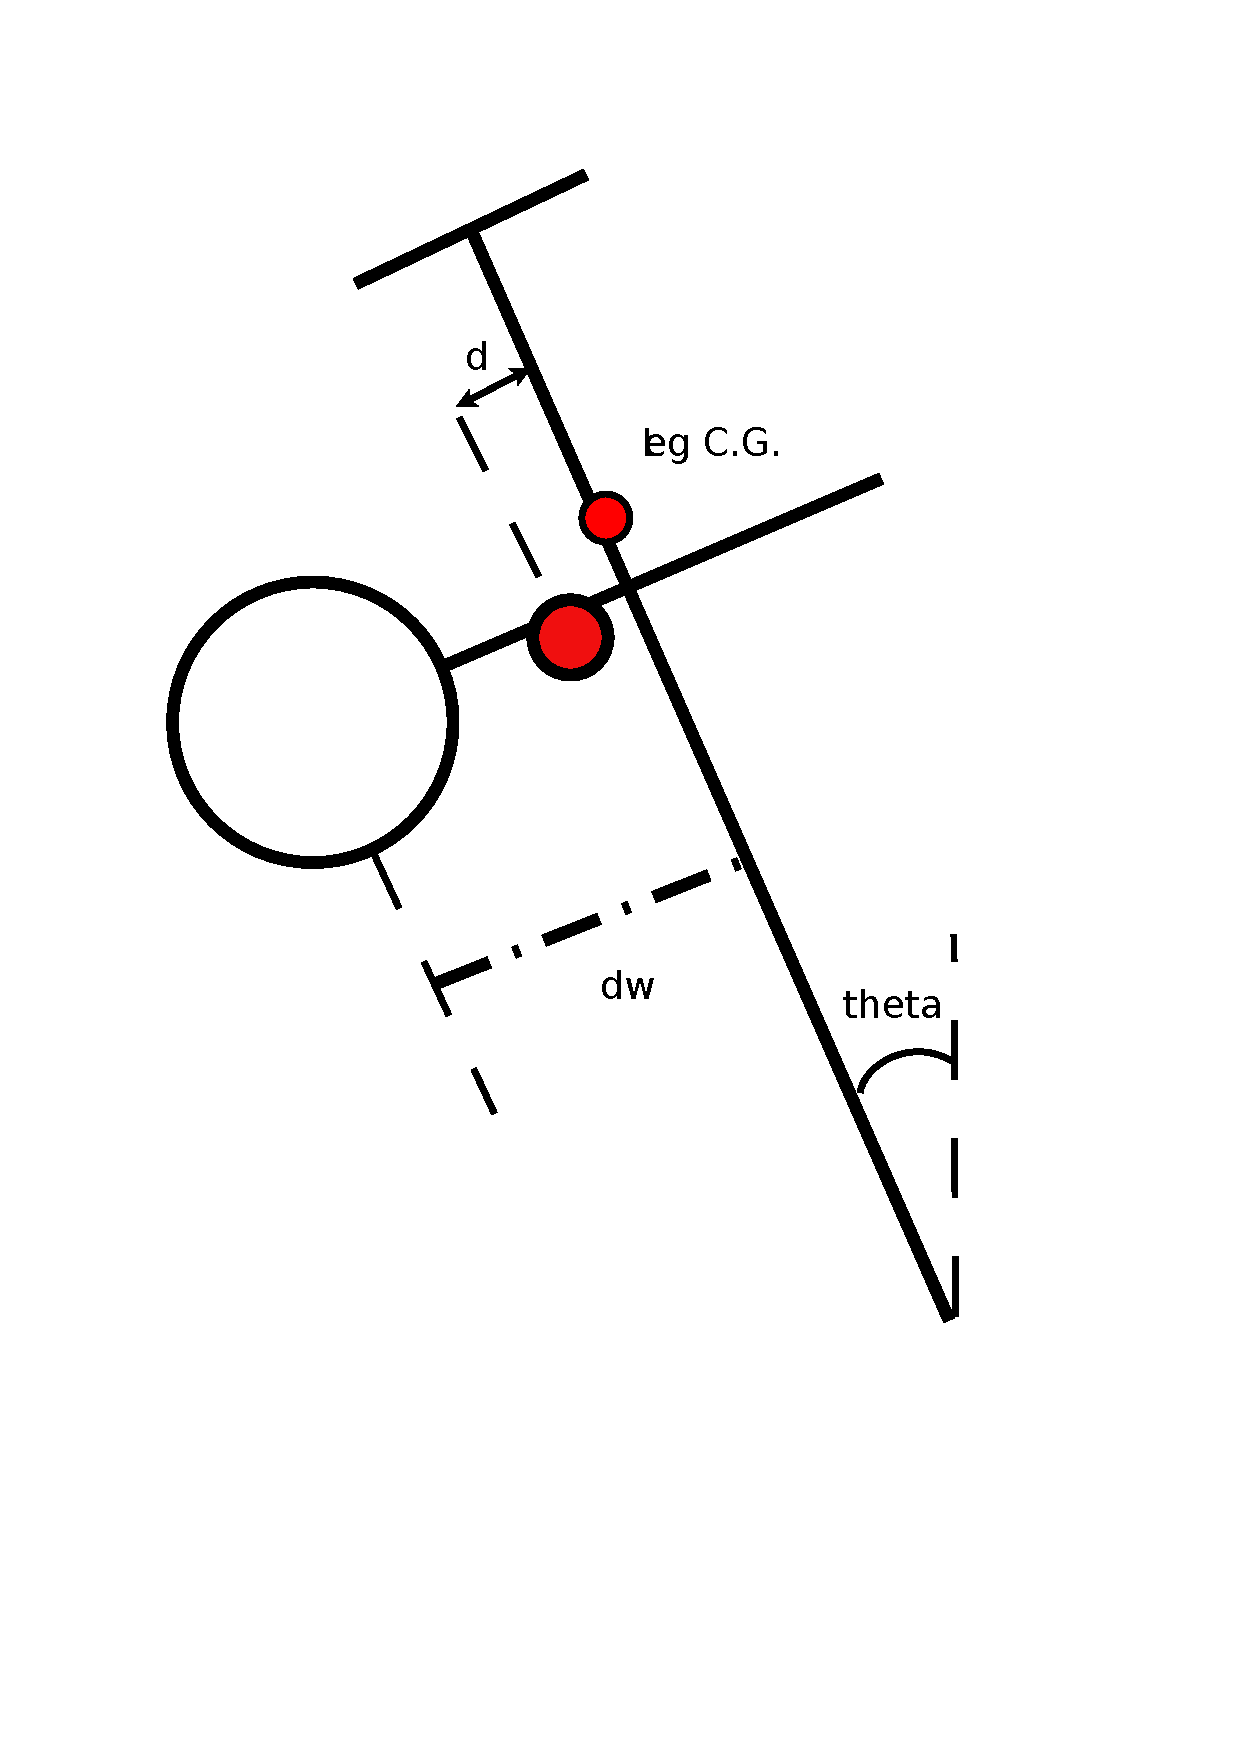
\includegraphics[scale=0.30]{fig/line_sketch.pdf}
\caption{Line sketch for the hopper}
\label{fig:4_line_sketch}
\end{figure}

We use the Euler--Lagrange equations derived from the Lagrangian as follows,
\begin{equation}
 T \:=\: \frac{1}{2}\:\:\left[\:\:m_w\:(\:\dot{x_w}^2 + \dot{y_w}^2\:) + m_p (\:\dot{x_p}^2 + \dot{y_p}^2\:)
  + m_l\:(\:\dot{x_l}^2 + \dot{y_l}^2\:) +  J_w\:(\:\dot{\phi} + \dot{\theta}\:)^2
  + J_b\:\dot{\theta}^2\:\:\right]
\end{equation}
\begin{equation}
V\:=\: g\:\left[\: m_l\:y_l\:+\: m_w\:y_w\:+\: m_p\:y_p\:\right] + \frac{1}{2}K\:(l - l_0)^2
\end{equation}
%\begin{equation}
% L = T - V
%\end{equation}
where,
\begin{eqnarray*}
x_l(t) &=& x(t) + \left[\:d - (\:l(t)- h\:)\:\:\tan \theta\:\right]\cos \theta\\
y_l(t) &=& x(t) + \left[\:l(t) - h \right]\:\:\cos \theta + d\:\:\sin \theta\\
\\
x_w(t) &=& x(t) - \:(\:d_w - d\:)\: \cos \theta\\
y_w(t) &=& y(t) - \:(\:d_w - d\:)\: \sin \theta
\end{eqnarray*}
\begin{eqnarray*}
x_p(t) &=& x(t) + d\: \cos \theta\\
y_p(t) &=& y(t) + d\: \sin \theta
\end{eqnarray*}

\vspace{0.2in}
\begin{tabular}{l @{ : } l}
$x_w$, $y_w$ & co-ordinates of the reaction wheel\\
$x_l$, $y_l$ & co-ordinates of the C.G. of the leg\\
$x_p$, $y_p$ & co-ordinates of the platform\\
$x$, $y$ & co-ordinates of the C.G. of the whole robot\\
$l(t)$ & length of the spring\\
$\theta$ & pitch angle measured as shown in the figure\\
$\phi$ & angle rotated by the reaction wheel relative to the robot\\
$d$ & distance of C.G. from the line of impact force\\
$d_w$ & distance of reaction wheel from the line of impact force\\
$l_0$ & non--extended length of the spring
\end{tabular}
\vspace{0.2in}

For co-ordinates of $q = \left[\:x(t)\;\;\;y(t)\;\;\;l(t)\;\;\;\theta(t)\;\;\;\phi(t)\:\right]$, we can derive the general equations of motion of the hopper by $L = T - V$,
\begin{equation}
\frac{d}{dt}\left(\frac{\partial\:L}{\partial\:\dot{q_A}}\right) - \frac{\partial\:L}{\partial\:q_A} = Q_A
\end{equation}
$Q_A$ is called the generalized constraint force. If 
\begin{equation}
 \psi_i(q) = 0,\;\; i = 1,\dots, m
\end{equation}
are $m$ constraint equations, we have,
\begin{equation}
 Q_A = \sum_{r=1}^m\lambda_r\;\frac{\partial \psi_r}{\partial q_A}
\end{equation}
We can divide the motion into three distinct stages,
\begin{center}
\vspace{0.2in}
\begin{tabular}{l p{4cm} @{ : } p{9cm}}
1. & Stance Phase & Foot in contact with ground, spring free to contract\\
2. & Flight Phase & Spring is being extended, no constraints used\\
3. & Spring Phase & Spring length constant
\end{tabular}
\vspace{0.2in}
\end{center}
Note that all algebra is solved symbolically in Mathematica. The equations thus derived are quite messy and hence not included in the report. The script to derive them is given in the appendix.
\section{Phases of motion}
Let us assume for some time that we do not have reaction wheel control and thus $\phi(t) = 0$ is always true. This is converted into another constraint for every phase of motion and used.
\subsection*{Stance Phase}
\label{subsec:4_stance_phase}
We define this phase from the moment the foot of the robot touches the ground till lift--off. Certain points to note are,
\begin{enumerate}
  \item
  Foot touches the ground when,
  \begin{equation}
  y(t) = (\;l(t_{impact}) - l_0\;)\:\cos \theta_{impact} + d \sin \theta_{impact}
  \end{equation}
  This is the condition when the previous phase i.e. spring phase ends.
  \item
  The impact torque acts upon the hopper C.G. We can find the moment arm of this torque and conserve angular momentum to get the final pitch rate.
  \begin{equation}
  arm = d \cos \theta + (\;l(t_{impact}) - l_0 - d \tan \theta\;)\;\sin \theta
  \end{equation}
  \begin{equation}
  \dot{\theta}_{new} = \dot{\theta}_{old} - (m_w + m_p + m_l)\; \frac{\dot{y}(t_{impact})\;arm}{J_b}
  \end{equation}

  \item
  The constraint equations for this are,
  \begin{eqnarray*}
    y(t) = (\;l(t) - l_0\;)\:\cos \theta + d \sin \theta\\
    x(t) = x_{f-impact} - (\;l(t) - l_0\;)\:\sin \theta - d \cos \theta
  \end{eqnarray*}
  where
  \begin{equation}
  x_{f-impact} =  x(t_{impact}) + (\;l(t_{impact}) - l_0\;)\:\sin \theta_{impact} + d \cos \theta_{impact}\\
  \end{equation}
  \item
  For deriving the equations, we follow a slightly different approach. Instead of solving for the Lagrange multipliers as described earlier, we can substitute these constraint equations in the Euler-Lagrange equations to get the final set of equations. Note that substituting them in the lagrangian is not correct as the derivation of E-L equations assumes that the variables are independent.
  \item
  Propagate the three differential equations thus obtained to stop using an event locator. We have designed the hopper in such a way that when the spring is at its normal length, the platform touches the top portion (from which springs are suspended). We want the platform to hit the robot with the maximum velocity to ensure maximum energy transfer. Hence, the event locator should stop the equation propagation at $l(t) = l_0$.
  \item
  We assume an inelastic collision between the platform and the robot i.e. they travel together after impact. This is ensured in the design by the ratchet and paul mechanism. Conserve momentum again to arrive at the final velocity of the robot.
%  \item
%  The stance phase propagator outputs all the states viz. $[\;x\;\;y\;\;l\;\;\theta\;\;\phi\;\;\dot{x}\;\;\dot{y}\;\;\dot{l}\;\;\dot{\theta}\;\;\dot{\phi}\;]$
\end{enumerate}

\subsection*{Flight Phase}
This stage is defined from lift--off till the spring extension is complete.
\begin{enumerate}
  \item
  Extension of the spring takes place during this phase. I have used a triangular velocity profile for
  the energy pumping motor. This means a constant positive and negative acceleration for the first half and the second half respectively.
  \begin{equation}
  \ddot{l}(t) = \left\{\begin{array}{ll}
			0 & l(t) \leq (l_0 - \epsilon)\;\;OR\;\;l(t) \geq (l_{max} + \epsilon)\\
			&\\
			l_{accel} & l_0 \leq l(t) \leq \frac{(l_{max} + l_0)}{2}\\
			&\\
			-l_{accel} & \frac{(l_{max} + l_0)}{2} \leq l(t) \leq l_{max}
                      \end{array} \right.
  \label{eqn:4_spring_retract}
  \end{equation}
  A buffer of $\epsilon$ is necessary because Mathematica uses floats and sometimes, the software calculates the value of $l(t)$ very close to $l_{max}$ and returns the comparison $l(t) == l_{max}$ as true even though there is a very small difference between them.
  \item
  We have used $\ddot{l}(t)$ in the control law. This means that the torque of the motor is being actuated. We need to convert this into a form that is implementable using the onboard rotatory encoders. This is done as follows,
  \begin{itemize}
    \item
    Start onboard time at lift-off. Calculate the desired velocity of the EPM motor according to Equation \ref{eqn:4_spring_retract}. This is the desired $\omega_d(t)$ of the motor. 
    \item 
    If $\omega(t)$ be the speed sensed by the encoders, we can devise a PID controller as,
    \begin{equation}
    e(t) = \omega(t) - \omega_d(t)
    \end{equation}
    \begin{equation}
    U_{l}(t) = K_w\;\omega_d(t) + K_p\;e(t) + K_d\;\frac{d\;e(t)}{dt} + K_i\;\int e(t)\;dt
    \label{eqn:4_l_controller}
    \end{equation}
    $K_w$ is the speed constant of the motor.
  \end{itemize}
  \item
  Flight equations are completely unconstrained.
  \item
  The event solver stops the propagation of flight equations when $l(t) = l_{max}$.
\end{enumerate}

\subsection*{Spring Phase}
This is the remainder of the hopper motion in air till the foot touches the ground.
\begin{enumerate}
  \item
  Spring length is constant during this phase. The constraint equation is therefore,
  \begin{equation}
  l(t) = l_{max}
  \end{equation}
  \item
  The event solver for spring phase stops integration when,
  \begin{equation}
  y(t) = (\;l(t) - l_0\;)\:\cos \theta + d \sin \theta
  \end{equation}
\end{enumerate}
Figure. \ref{fig:4_eqn_prop} shows these equations being used to together to generate a hopping gait. We 
have started the hopper from a good initial condition arrived at by methods discussed in later sections 
and the figure shows the trajectory of the C.G. during the motion. Figure \ref{fig:4_spring_paramsG} shows 
the variation of states during the Spring Phase. It is seen that attitude re--orients itself due to SLOM 
effect during this.
\begin{figure}[!htp]
\centering
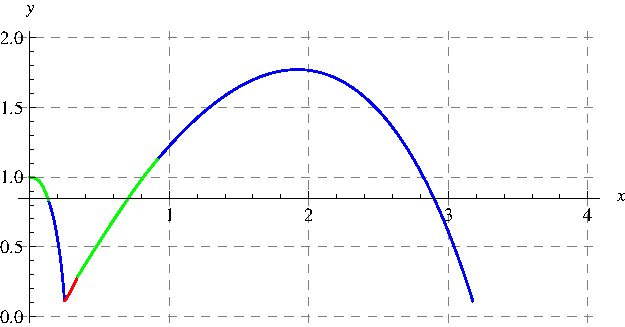
\includegraphics[scale=1.5]{fig/plotG.pdf}
\caption[Propagation of equations of motion]{Propagation of equations of motion : Flight Phase - Green, Spring Phase - Blue, Stance Phase - Red, distances in meters}
\label{fig:4_eqn_prop}
\end{figure}

\begin{figure}[!htp]
\centering
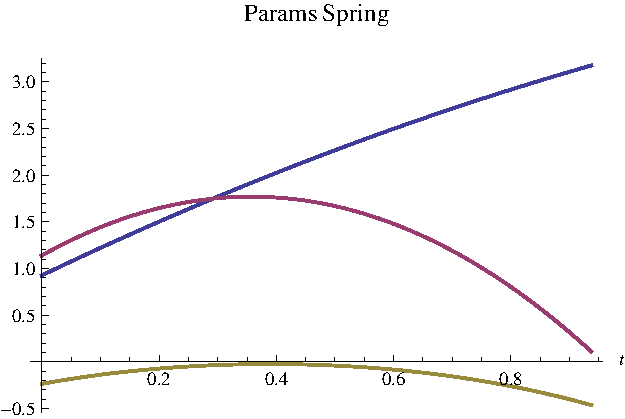
\includegraphics[scale=1]{fig/pSpringParamsG.pdf}
\caption{Spring Phase parameters : $x(t)$ - Blue, $y(t)$ - Pink, $\theta(t)$ - Yellow, t = secs}
\label{fig:4_spring_paramsG}
\end{figure}

\section{In-place hopping}
It is difficult for SLOM system to perform inplace hopping. The impact torque is a destabilizing one and hence active control is necessary for inplace hopping. Figures \ref{fig:4_inplace_trajec}, \ref{fig:4_inplace_flight_params} and \ref{fig:4_inplace_stance_params} show the performance of the controller described below for inplace hopping.
\begin{enumerate}
 \item
  The basic characteristic of the controller will have to be that it should always keep the attitude of the robot constant. The value of this constant attitude needs to be found out by a detailed analysis. We would like to take into account the energy spent by the controller to keep the attitude constant inorder to decide the value of the desired attitude. The cost metric can be the deviation of the horizontal distance in successsive hops and the energy consumed ($\dot{\theta}\;\ddot{\theta}$). I decided to keep the attitude constant to zero for the time being.
  \item
  The flight and spring phases consist of a simple PID controller that re-orients the attitude to bring it to zero. Figure \ref{fig:4_inplace_flight_params} shows its performance after the hopper is released with an attitude of $1 rad$. The controller manages to quickly correct the attitude.
\begin{figure}[H]
\centering
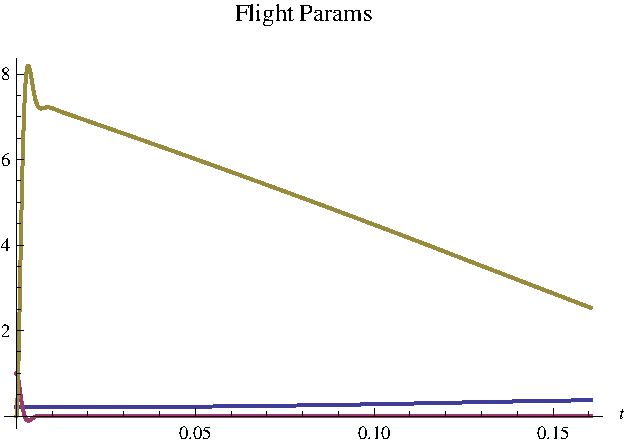
\includegraphics[scale=0.8]{fig/inplace_pFlight_params.pdf}
\caption{Inplace Flight Phase parameters : $l(t)$ - Blue, $\theta(t)$ - Pink, $\phi(t)$ - Yellow, t = secs}
\label{fig:4_inplace_flight_params}
\end{figure}

  \item
  The stance phase controller is slightly different. It was observed that if the desired attitude was zero in the stance phase also, the hopper slowly starts to drift backwards in successive hops. This is rectified by giving the desired attitude after the stance phase as,
  \begin{equation}
   \theta_d = \tan^{-1}\left(\frac{x_{impact}}{h_{max}}\right)
  \end{equation}
  \item
  This ensures that the hopper always tries to go towards $x = 0$ position and thus performs satisfactory inplace hops. The performance of the stance controller is shown in Figure \ref{fig:4_inplace_stance_params}
  \begin{figure}[!htp]
\centering
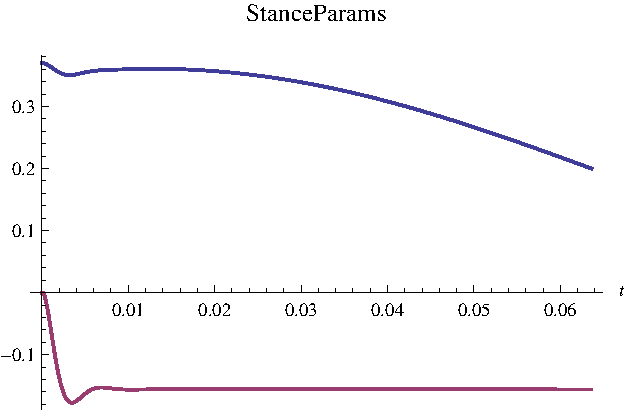
\includegraphics[scale=1]{fig/inplace_pStance_params.pdf}
\caption{Inplace Stance Phase parameters : $l(t)$ - Blue, $\theta(t)$ - Pink, t = secs}
\label{fig:4_inplace_stance_params}
\end{figure}

\end{enumerate}

\begin{figure}[!htp]
\centering
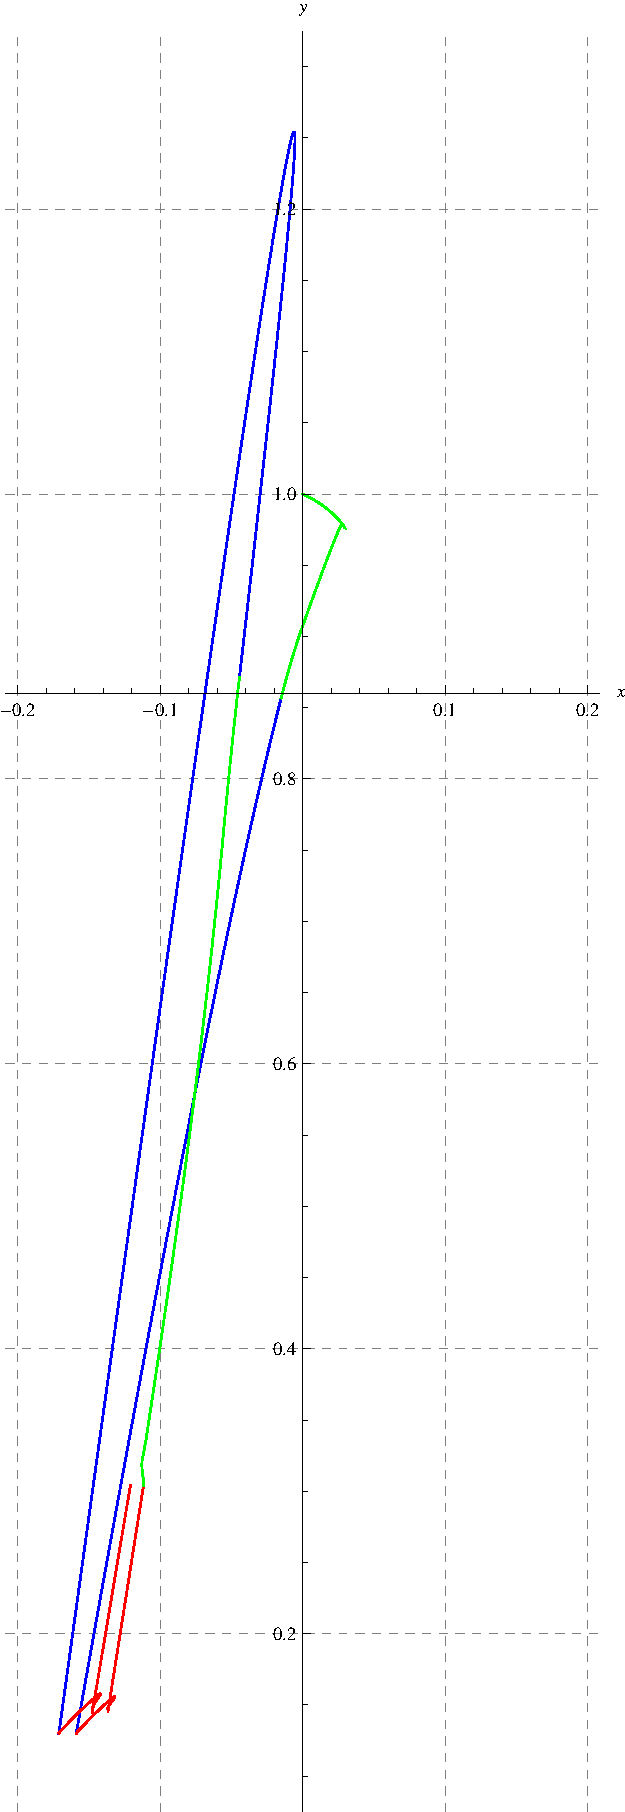
\includegraphics[scale=0.6]{fig/plot_inplace.pdf}
\caption[Trajectories of two inplace hops]{Trajectories of two inplace hops : Flight Phase - Green, Spring Phase - Blue, Stance Phase - Red, distances in meters}
\label{fig:4_inplace_trajec}
\end{figure}


\section{Stable gait}
\begin{figure}[H]
\centering
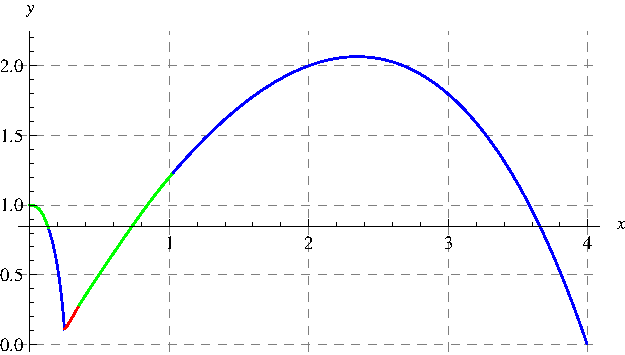
\includegraphics[scale=0.8]{fig/plot_perturb.pdf}
\caption{Propagation of equations of motion with $\Delta\;\dot{\theta}(t) = 0.05\;rad/s$}
\label{fig:4_eqn_perturb}
\end{figure}
Figure. \ref{fig:4_eqn_perturb} shows the change in trajectory after a small perturbation in the initial 
conditions at $t = 0$ i.e. at $x = 0$ in $\dot{\theta}$. Note that the maximum height is significantly 
higher and the height of the second impact point is almost zero, this suggests a very bad pitch attitude 
of the robot as is verified by Figure. \ref{fig:4_spring_params_perturb}. The hopper falls flat on its 
face!
\begin{figure}[!htp]
\centering
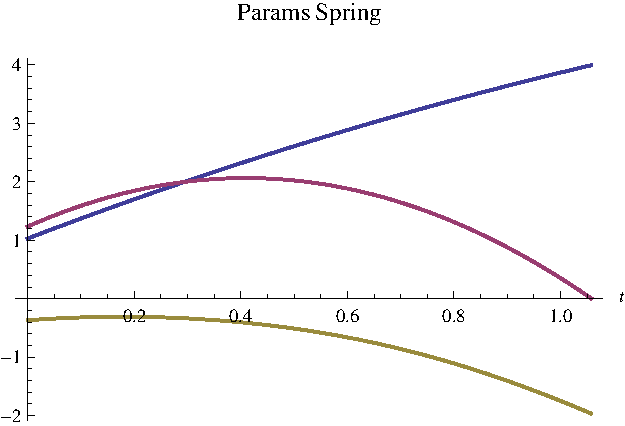
\includegraphics[scale=0.8]{fig/pSpringParams_perturb.pdf}
\caption{Spring Phase parameters : $x(t)$ - Blue, $y(t)$ - Pink, $\theta(t)$ - Yellow, t = secs}
\label{fig:4_spring_params_perturb}
\end{figure}
Thus, our next aim is to find out a set of initial conditions such that the states at the point of impact at successive hops do not differ by much. We define the measure of the change in the impact states by taking the norm of the states $q_A$ and $q_B$,
\begin{equation}
norm = \sum_{i = 1, i\;\neq\;1, 5, 10}^{10} || q_{A_i} - q_{B_i} ||
\end{equation}
where $q = [\;x\;\;y\;\;l\;\;\theta\;\;\phi\;\;\dot{x}\;\;\dot{y}\;\;\dot{l}\;\;\dot{\theta}\;\;\dot{\phi}\;]$ and we remove $x(t)$, $\phi(t)$ and $\dot{\phi}(t)$ from the norm. 

\subsection*{Good initial conditions}
The only thing we can control is the initial conditions at the launch. Everything after that is a product of the propagation of differential equations. We try to find a stable gait as follows,
\begin{enumerate}
  \item
  Keep desired parameters as a hopping height of 1 m and horizontal velocity of 1 m/s. Start propagation 
  of the equations from the topmost point of the trajectory, i.e. $x = 0$, $\dot{x} = 1$, $\dot{y} = 0$ 
  and $y = 1$. $\phi$ and $\dot{\phi}$ are of course both zero.
  \item
  Now we have $l_{max}$, $\theta_0$ and $\dot{\theta}_0$ as the three parameters which we can vary.
  \item
  Since we are neglecting friction in all the above analysis, we can calculate the amount of energy lost in the impact and thus the energy needed to be put into the system each hop. This gives, $l_{max} = 0.37 m$.
  \item
  We now try to run an optimizing algorithm to get optimal states at the launching instant as shown in \cite{ga_init}. Let the attitude of the robot be zero at the launch. This fixes $\theta_0$. The only parameter left to be varied is $\dot{\theta}_0$.
  \item
  We are using Mathematica to compute all this. There are a host of problems associated with it. It is slow to propagate the equations and they also become stiff at certain initial conditions when the solver fails. 
  \item
  An optimizer will try to find a global minima for the objective function (using the internal NMinimize method) which is the minimization of norm in our case. It needs to compute these equations for a lot of different initial conditions quickly which Mathematica cannot do. Different approaches like Genetic Algorithms other than the default built-in optimization routine are also equally slow.
  \item
  On top of this, the problem with our system is that it is a very rapidly changing system. There are a lot of local minimas very near to each other. NMinimize gets stuck in these minimas and it jumps out of one to get stuck in the neighbouring one.
  \item
  So instead of using NMinimize to find states such that the norm goes to zero, I tried to iterate over the region manually. By oberserving the norm at each stage, I found out a few sets where the norm was small enough to be taken care of by the controller. The trajectory generated by these conditions is showed in Figure \ref{fig:4_eqn_prop}.
\end{enumerate}

\section{Poincare Map}
It is known that our system is a highly non-linear periodical dynamical system. Poincare Map of \textit{ first return map} is one classical tool to study the dynamics of periodic systems. Consider a set of autonomous differential equations,
\begin{equation}
 \frac{d {\bf x}}{d t} = \dot{{\bf x}} = f({\bf x})
\label{eq:4_poincare}
\end{equation}
where ${\bf x} = {\bf x}(t) = [x_1,\;...\;,x_n]$ is the state vector of independent variables. $f : \mathcal{U} \to \mathcal{R}^n$ where $\mathcal{U} \subseteq \mathcal{R}^n$. Let $\phi_t({\bf x}) = \phi({\bf x}, t)$ be a flow generated by vector field $f$ and satisfies Equation \ref{eq:4_poincare}. An initial condition is ${\bf x}_{in} = {\bf x}(0)$ and the corresponding solution is $\phi({\bf x}_{in}, t)$ with $\phi({\bf x}_{in}, 0) = {\bf x}_{in}$.

We now have two curves, a solution curve that propagates the solution given an initial condition ${\bf x}_{in}$ and an orbit curve which is a set of all the states taken by this solution curve. The kind of solutions we are interested in are,
\begin{equation}
 f(\bar{{\bf x}}) = 0
\end{equation}
This is the fixed point of the solution which might have the following characteristics,
\begin{enumerate}
  \item
  The solution might start in the neighbourhood of $\bar{\bf x}$ and continue to remain near it. This is called a \textit{stable} solution.
  \item
  The solution might converge asymtotically towards $\bar{\bf x}$ to give an \textit{aymsptotically stable} solution.
  \item
  It can diverge from $\bar{\bf x}$ if $\bar{\bf x}$ is an unstable solution.
\end{enumerate}
We can thus see that a Poincare Map converts a $n^{th}$ order dynamical system into a $(n-1)^{th}$ order discrete system. It is almost perfect for our analysis. We can examine the periodicity and the stability of the locomotion with the help of this map.\\

Let $\gamma$ be a closed orbit of the $n$ dimensional system. Find a local cross-section about $\gamma$ of dimension $(n-1)$ and let it be $\Sigma$. $\Sigma$ is the (n-1) dimensional hyper-surface. It need not be planar but has to be transverse to $\gamma$. Consider a point $\bf p$ on $\Sigma$. All orbits near $\gamma$ have to pass through $\Sigma$. If we define $\Sigma$ such that it is a smooth scalar function $g : \mathcal{R}^n \to \mathcal{R}$, we can say,
\begin{equation}
\Sigma = \lbrace {\bf x} \in \mathcal{R}^n : g({\bf x}) = 0 \rbrace
\end{equation}
The condition on $g$ is just that
\begin{equation}
\nabla g({\bf p})^T f({\bf p}) \neq 0 
\end{equation}
i.e. the gradient is not orthogonal to the flow at point $p$. 
\begin{figure}[!htp]
\centering
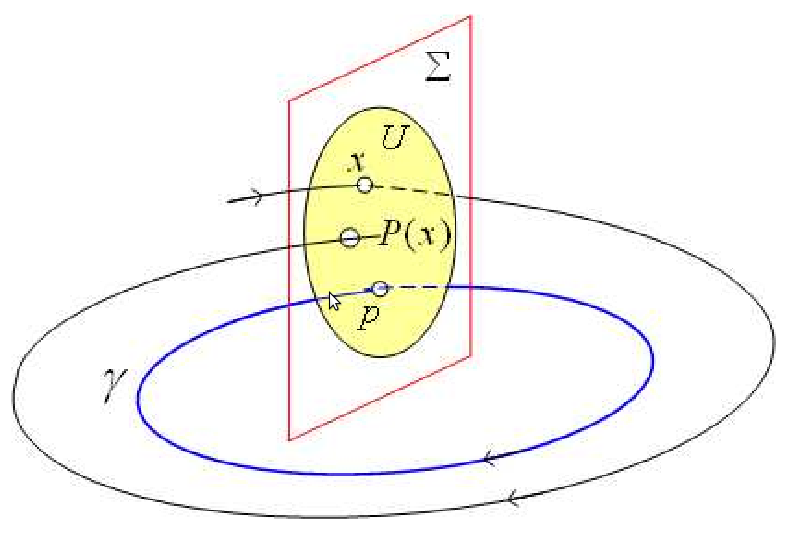
\includegraphics[scale=1.4]{fig/poincare.png}
\caption[Poincare Map : Schematic]{Poincare Map : Schematic \cite{sayyad}}
\label{fig:4_poincare}
\end{figure}
Let $\mathcal{U}$ be a neighbourhood of $p$ such that $\gamma$ intersects $\Sigma$ only once in the neighbourhood. We define the Poincare map from $\mathcal{U} \to \mathcal{R}^n$ as,
\begin{equation}
{\bf P (x)} = \phi_{\tau}({\bf x})
\end{equation}
$\phi_{\tau}$ is the flow of the system. As the point ${\bf x} \to {\bf p}$, $\tau \to T$ which is the return period of the system at ${\bf p}$. Thus, we can say,
\begin{equation}
{\bf x}_{k+1} = {\bf P} ({\bf x}_k)
\end{equation}
If the Jacobian of this map,
\begin{equation}
{\bf J}_{\bf p} = \frac{d\;\;{\bf P(x)}}{d {\bf x}}\;\;at\;\;{\bf x = p}
\end{equation}
has all its eigenvalues inside the unit circle, the point $\bf p$ is a stable point.\\

For our system, we try to find a map between successive impact states. The fixed point of the map will be 
an equilibrium point and can be analysed for stability. The Poincare Map is thus a routine which takes in 
${\bf x}_k$ and gives out ${\bf x}_{k+1}$ after propagating the differential equations.\\

The optimization 
procedure described above also aims to find the fixed point. So using exactly similar procedure, we arrive 
at a set of states such that the robot hops for around 2 hops without falling. Note that this is not the 
exact fixed point, it has been been arrived at manually. We perturb the initial states by a small amount 
to see that the final impact states change drastically. Hence, this is in the neighbourhood of an unstable 
fixed point. Due to issues mentioned above, I have not been able to find a stable fixed point for the 
hopper. All the points I found have non-zero values of norms although they are very small.\\
\vspace{0.1in}

\lstinputlisting{poincare_code.m}

\section{Control Strategies}
We have the reaction wheel and the spring length as two control variables. The control of spring length is 
done as described in Section \ref{subsec:4_stance_phase}. We look at orientation control in this section. We would like to achieve trajectory following using orientation control. 
\subsection*{Stance Phase}
A few points to be noted are,
\begin{enumerate}
  \item
  Stance Phase is the most important phase for trajectory following. A bad attitude at lift-off results in a totally different trajectory in space and mere orientation control is obviously not enough to follow it.
  \item
  We decide to follow the time series of attitude values during stance phase. Stance times are small, about 30-40 msecs. The control procedure is as follows,
  \begin{itemize}
    \item
    Generate a time series of the attitude using the good launch parameters and call it $\theta_G(t)$. Perturb the launch parameters by a small amount and start the integration to get a time series $\theta(t)$.
    \item
    Define,
    \begin{equation}
      e(t) = \theta(t) - \theta_G(t)
    \end{equation}
    This gives $\frac{d e}{d t} = \dot{\theta}(t) - \dot{\theta}_G(t)$.\\ We also put in the integral gain as $iErr = \sum e$. It is ensured that,
      \begin{equation*}
	-iErrMax\;\;\leq\;\;iErr\;\;\leq\;\;iErrMax
      \end{equation*}
    \item
    The control input is given as,
    \begin{equation}
     \ddot{\phi}(t) = K_p\;e + K_d\;\dot{e} + K_i\;iErr
    \end{equation}
  \end{itemize}
  \begin{figure}[!htp]
  \centering
  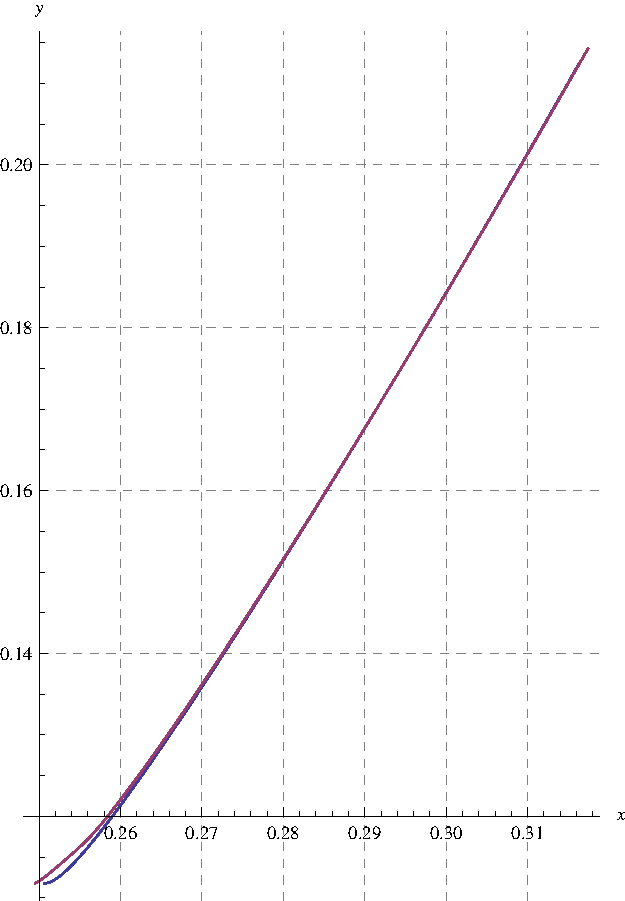
\includegraphics[scale=1]{fig/pStance_trajec_control.pdf}
  \caption{Stance Controller : Good trajectory - Blue, Perturbed trajectory - Pink, distances in meters}
  \label{fig:4_stance_control_trajec}
  \end{figure}

  \begin{figure}[!htp]
  \centering
  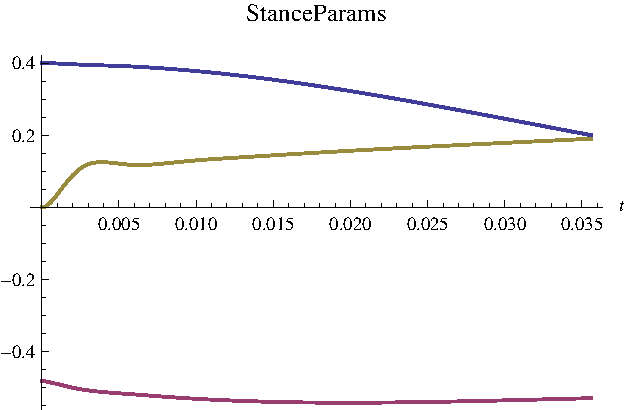
\includegraphics[scale=1]{fig/pStance_params_control.pdf}
  \caption{Stance Controller variables : $l(t)$ - Blue, $\theta(t)$ - Pink, $\phi(t)$ - Yellow, t = secs}
  \label{fig:4_stance_control_var}
  \end{figure}

  \item
  A few problems in the control strategy are apparent. The stance times of the good trajectory and the 
  control trajectory will not be equal. Hence, a PID controller based upon the comparison on the time 
  series will not always work.
\end{enumerate}

\subsection*{Flight and Spring Phases}
\begin{enumerate}
  \item
  It was noted that the perturbed trajectories in the flight and spring phases are significantly different than the good ones. This is due to the large time scales associated with them, around 400--500 msecs.
  \item
  We need a different control strategy for two reasons, firstly a slight error at liftoff causes a different trajectory in space and trajectory following breaks down, secondly due to the reason mentioned above.
  \item
  \begin{figure}[H]
  \centering
  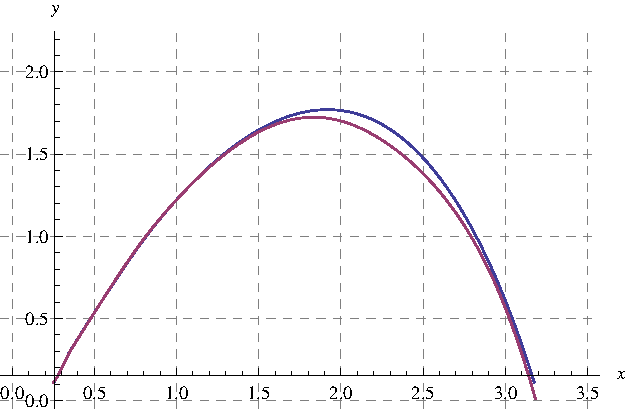
\includegraphics[scale=1.1]{fig/pFullTrajec_control.pdf}
  \caption[Trajectory Controller : Good - Blue, Perturbed - Pink]{Trajectory Controller : Good - Blue, Perturbed - Pink, Note that the trajectories deviate significantly after the flight phase resulting in a relatively bad attitude at impact.}
  \label{fig:4_full_trajec_control}
  \end{figure}

  I tried out a different control law viz.
  \begin{itemize}
    \item 
    Solve the attitude re--orientation problem at every instant when the control input gets calculated to ensure that the hopper lands on the ground with the same attitude as that of the previous hop.
    \begin{equation}
     y_{impact} = (l(t_{impact}) - l_0)\;\cos \theta_{impact} - d \sin \theta_{impact}
    \end{equation}
    \item  
    Find the time left for impact $t_{left}$ as a solution of,
    \begin{equation}
     y_{impact} - y(t) =  \dot{y}(t)\;t - \frac{1}{2}\;g\;t^2
    \end{equation}
    \item
    Find the displacement in $\theta$ to impact with the correct attitude and give the corresponding torque command to the controller,
    \begin{equation}
     \Delta\;\theta (t)= \theta_{impact} - \theta(t)
    \end{equation}
    \begin{equation}
    \ddot{\phi}_d(t) = \left(\frac{-2\;J_b}{J_w}\right) \left(\frac{\Delta\;\theta - \dot{\theta}(t)\;t_{left}}{t_{left}^2}\right)
    \end{equation}
    \item
    This is the reference signal for the controller. We put a PID controller on top of this where the error is taken as,
    \begin{equation}
     e(t) = \ddot{\phi}(t) - \ddot{\phi}_d(t)
    \end{equation}
    \begin{equation}
     U_{\phi}(t) = \ddot{\phi}_d(t) + K_p\;e(t) + K_d\;\dddot{\phi}(t) + K_i\;\;iErrPhi
    \end{equation}
    as done in the spring extension controller. This is again a torque controller and needs to be converted into a velocity controller as done in Equation \ref{eqn:4_l_controller}.
  \end{itemize}
  \item
  As shown in Figure \ref{fig:4_full_trajec_control}, the controller manages to follow the trajectory pretty well. However, the attitude at the end of the perturbed trajectory is quite bad. Further refinement in control strategy is necessary to improve performance.
\end{enumerate}









